\newcommand{\figureLCDCharRow}[1]{
  \def\lang{\detokenize{#1}}
  \def\langRu{\detokenize{ru}}
  \def\langEn{\detokenize{en}}
  \def\figureCaption{XXX: No translation.}
  \ifx \lang\langRu
  \def\figureCaption{
    Кодирование пикселей в одной строке символа текстового ЖК-дисплея.
  }
  \fi
  \ifx \lang\langEn
  \def\figureCaption{
    Pixel encoding in one row of a char on an text LCD.
  }
  \fi
  \begin{figure}[ht]
    \centering
    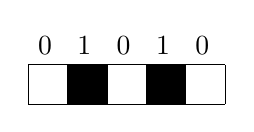
\begin{tikzpicture}
      \draw[step=0.5cm,black,very thin] (-2.5, -0.5) grid (0, 0);
      \fill[black] (-2.0, 0) rectangle (-1.5, -0.5);
      \fill[black] (-1.0, 0) rectangle (-0.5, -0.5);
      \foreach \x/\n in {-2.5/0, -2.0/1, -1.5/0, -1.0/1, -0.5/0} {
        \draw (\x cm, 0) node[anchor=south west] {$\n$};
      }
    \end{tikzpicture}
    \caption{\figureCaption}
    \label{fig:game-dev-char-symbol-encoding}
  \end{figure}
}
